Na klastre bolo aplikované viacnásobné zarovnanie.
\begin{lstlisting}[language=Python, caption={Clustering without primers}, label={lst:python-clustering-without-primers}]
ClusterFile = TextFileM(path="clusters_output.txt")
ClusterFile = ClusterFile.load()
ClusterFile = parse_tuple_file(ClusterFile)
ClusterFile = get_clusters(ClusterFile)
clusters = ClusterFile.data

#ClusterFile = pick_largest_cluster(ClusterFile)
#LargestCluster = []
#LargestCluster = ClusterFile.data

clusters = [l for l in clusters if len(l) > 10]
count=1
for clust in clusters:
    ClusterFile.data=clust
    ClusterFile = retrieve_dna_lines(ClusterFile, clover_input_path)
    DataToBeAligned = ClusterFile.data

    ClusterSize = len(DataToBeAligned)
    (Aligned, Unaligned) = DataBeamAlgorithmSplit(DataToBeAligned, 10)
    dist = len(Aligned[0].replace("_",""))
    if len(Aligned[0].replace("_",""))<10:
        continue

    Aligned.insert(0,str(clust))

    TextFileM(data=Aligned).write_data_to_file(f"GeneratedData/Aligned_dnaSize-{dist}num-{ClusterSize}id-{count}.txt")
    count+=1
\end{lstlisting}
Filtrovaním klastrov na vacsie ako 10 sekvencií bolo dosiahnuté, že sa zarovnávali iba klastre s dostatočným počtom sekvencií, čo umožnilo získať robustnejšie výsledky.
Taktiež bolo odfiltrované zarovnanie klastrov, ktoré obsahovali sekvencie s dĺžkou kratšou ako 10 nukleotidov, aby sa zabezpečilo, že zarovnávané sekvencie budú dostatočne dlhé na získanie zmysluplných výsledkov.
Ukázalo sa, že klastre obsahovali sekvencie, ktoré mali zhodu nielen na začiatku, ale aj ďalej v reťazci.
Niektoré klastre obsahovali sekvencie, ktoré sa zhodovali až do dĺžky 100 nukleotidov, čo predstavuje výrazne dlhší úsek než pôvodný primér.

\subsubsection*{Príklad získaného zarovnania}

Na obrázku \ref{fig:zarovnane_retazce} je zobrazený príklad jedného z mnohých nájdených zarovnaných klastrov. Vidno, že jednotlivé čítania obsahujú spoločné úseky, ktoré boli úspešne zarovnané, čo potvrdzuje správnosť detekcie priméru a klastrovania.

\begin{figure}[htbp]
\centering
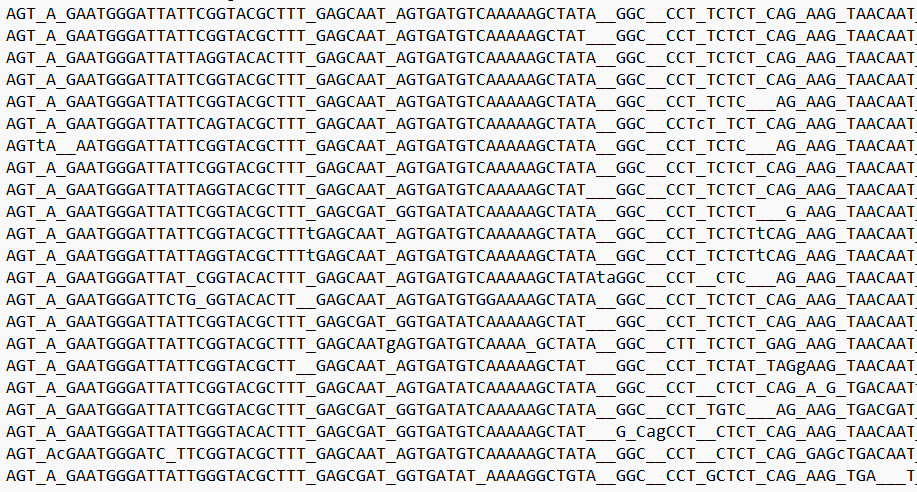
\includegraphics[width=0.95\textwidth]{chapters/Figures/ZarovnaneRetazce}
\caption{Príklad zarovnania DNA sekvencií z jedného klastra. Obrázok ukazuje konzenzuálne výsledky viacnásobného zarovnania s viditeľnými zhodami v sekvenciách.}
\label{fig:zarovnane_retazce}
\end{figure}
